\subparagraph{Low critical node degree, KANSKJE FJERNE DETTE HER OG neste subpara}
To explain why a network where the critical node degree is set to a low degree, ends up in a clique, 
 lets consider the variables and their values shown in (table \ref{tbl:clique}), $n$ is the number of nodes. With these values, Eq.(\ref{eq:discountstar}) is satisfied until a node is considering establish its third direct link. At this point the node has reached the critical degree, and will strictly prefer to establish direct links. This will lead to even more nodes reaching the critical degree level, and the result is that almost every node connects to every one else. Two of the resulting simulating networks with these parameters can be seen in Figure \ref{fig:discounthighdegree}. As we can see from the parameters in table \ref{tbl:clique}, the critical degree is reached when a node gets a degree of two. From degree two and up, $c<\beta-\beta^{2}$. The expected number of nodes with degree of two are $E(g=2)=10*2^{-2}=2.5$. This is when we assume that the network follow a power-law with $\gamma=2$.
\begin{table}[h]
\centering
\begin{tabular}{lc}
 \hline
  $
  n=10,
  \beta=0.7,
  \beta-\beta^2=0.21,
  I_{l}=0.6$\\
  \hline
\end{tabular}
\caption{The parameters used in the simulation in \ref{fig:stablestar} \label{tbl:clique}}
\end{table}





\subparagraph{High critical node degree}
To ensure that the network will form a star, we have to find parameters such that, Eq.(\ref{eq:discountstar}) is satisfied, and the probability of a node having a critical degree has to be relative low. In a network with ten nodes, the expected number of nodes with degree five in a network with ten nodes, is $E(g=5)=10*5^{-2}=0.4$. With the parameters from table \ref{tbl:discountstar}, these conditions are satisfied and the resulting network can be seen in Figure \ref{fig:star:a}.
  
\begin{table}[h]
\centering
\begin{tabular}{lc}
 \hline
  $
  n=10,
  \beta=0.8,
  \beta-\beta^2=0.16,
  I_{l}=0.7$\\
  \hline
\end{tabular}
\caption{The parameters used in the simulation in \ref{fig:star:a} \label{tbl:discountstar}}
\end{table}


\
\
......FROM HERE, it's only notes.......
\section{DETTE ET ANNET STED KANSKJE? BLIR LITT RART Å HOPPE INN I DET HER}
By adjusting the parameter one can assure that only insured agents connects to other insured agents, and the opposite,
that only uninsured agents connects to each other. Hence as we can see from the Figure \ref{fig:fincont} clustered
networks of insured agents (red) are created, and  as the paper \cite{contagion} showed, these clustered trusted
networks, can achieve higher, super-critical, payoff by increasing their node degree past the critical point.

\begin{figure}[h]
\centering
\begin{subfigure}{.5\textwidth}
  \centering
  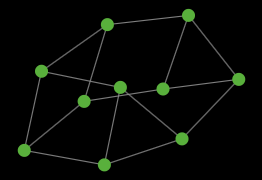
\includegraphics[width=0.8\linewidth]{../Figures/financialContagion1.png}
  \caption{\label{fig:fincont1} Initial graph with 10 agents.}
\end{subfigure}
\quad
\begin{subfigure}{.46\textwidth}
  \centering
  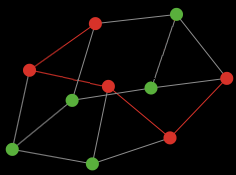
\includegraphics[width=0.8\linewidth]{../Figures/financialContagion2.png}
  \caption{\label{fig:fincont2} Insured agents (red) forms a network}
\end{subfigure}
\caption{\label{fig:fincont} shows how insured agents connects with each other to form a network to achieve super-critical payoffs.}
\end{figure}

, because the nodes can thus receive a super-critical payoff, and they are also insured against contagious risk.  

Figure \ref{fig:GTmodel1equations} presents the individual payoffs in a formation game between two agents in the described model. It is assumed that both agents has to have a desire to establish a connection in order to create a link between them. This is reasonable since a company would not prefer to enter into an agreement with negative expected payoff. As in this case would be the result when an insured agent is requested a connection with someone without insurance. 
 
 
\begin{figure}[h]
\centering
\begin{tabular}{@{}c@{}}
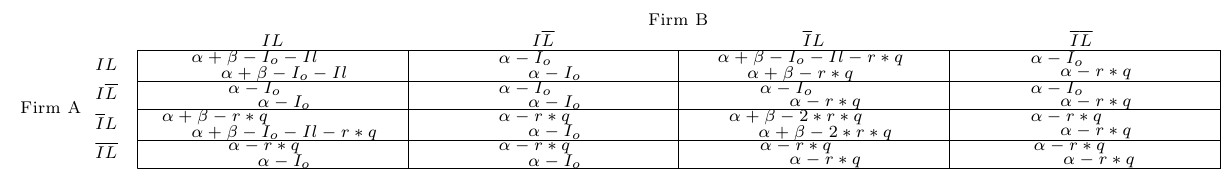
\includegraphics[width=1.0\textwidth]{../Figures/gameTheoryModel1WithEquations.png}
\end{tabular}
\caption[Caption for LOF]{\label{fig:GTmodel1equations} Normal form game between two agents individually choosing to purchase insurance and express desire to connect to the other  \footnotemark }
\end{figure}
\footnotetext{A link will only be created if both agents wishes to establish a connection.}

If we give value to the variables in Figure \ref{fig:GTmodel1equations} one can observe the model's different equilibrium's. It is difficult to know exactly how the variables are set and this would vary considerably between different markets. In a real worlds scenario the variables would also be different for each agent. However in Figure \ref{fig:GTmodel1} we decided to set a fixed value (which is assumed to be corresponding to the real values) for each variable in order to show a concept of how cyber-insurance can be used to create beneficial payoffs.
The following values where used: $\alpha$ = 10, $\beta$ = 10, $I_{o}$ = 5, $I_{l}$ = 2, $r$  = 20, $q$ = 0.5.


\begin{figure}[h]
\centering
\begin{tabular}{@{}c@{}}
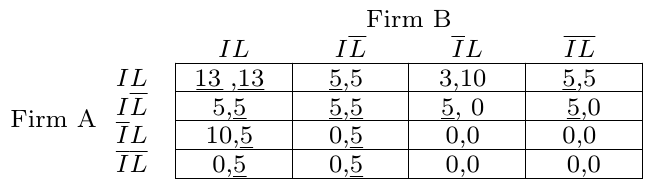
\includegraphics[width=0.6\textwidth]{../Figures/gameTheoryModel1WithNumbers.png}
\end{tabular}
\caption{\label{fig:GTmodel1} Shows equilibrium's in the resulting payoff matrix.}
\end{figure}

From the payoff matrix \ref{fig:GTmodel1} we observe two different Nash equilibrium's: One when both agents are insured and wants to connect to the other agent, and one when both are insured but does not want to establish a connection. These are the possible outcomes between the two agents, however as we can see it the social optimal solution would be for two insured agents to connect with each other, i.e they would both receive a significantly higher payoff. This demonstrates that a cluster of insured nodes would achieve higher payoffs.  
